\documentclass[tikz,border=5pt]{standalone}
\usepackage[T1]{fontenc}
\usepackage{lmodern,amsmath,amssymb}
\usetikzlibrary{arrows.meta,calc,positioning,fit,backgrounds,shapes.geometric,matrix,decorations.pathreplacing,patterns}
\definecolor{ink}{gray}{0.08}
\definecolor{wash}{gray}{0.965}
\definecolor{soft}{gray}{0.45}
\tikzset{box/.style={draw=ink,line width=.65pt,fill=white,align=center,inner sep=4pt,outer sep=0pt,font=\small},flow/.style={draw=ink,line width=.65pt,-{Latex[length=1.8mm,width=1.3mm]},rounded corners=2pt},annotation/.style={font=\scriptsize,text=soft,align=center},groupbox/.style={draw=soft,dashed,line width=.45pt,fill=wash}}
\begin{document}
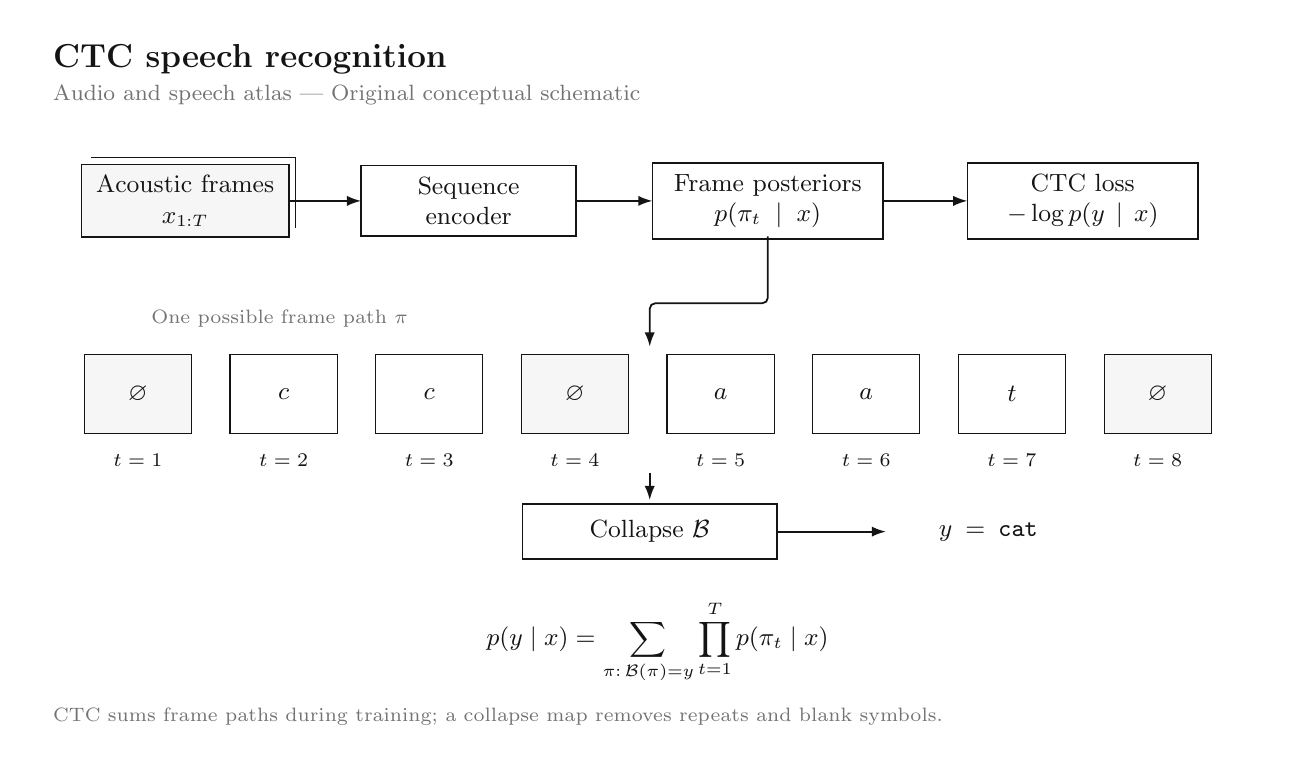
\begin{tikzpicture}[x=1cm,y=-1cm,font=\rmfamily,text=ink]

\path[use as bounding box] (0,0) rectangle (16,9);
\node[anchor=west,font=\large\bfseries] at (.2,.4) {CTC speech recognition};
\node[anchor=west,font=\footnotesize,text=soft] at (.2,.85) {Audio and speech atlas | Original conceptual schematic};
\begin{pgfonlayer}{background}
\end{pgfonlayer}
\node[box,fill=wash,minimum width=2.6cm,minimum height=0.9cm,text width=2.35cm] (input) at (2,2.2) {Acoustic frames\\$x_{1:T}$};
\draw[ink,line width=.4pt] (0.7999999999999999,1.6500000000000001) -- (3.4,1.6500000000000001) -- (3.4,2.5500000000000003);
\node[box,minimum width=2.7cm,minimum height=0.9cm,text width=2.45cm] (encoder) at (5.6,2.2) {Sequence encoder};
\node[box,minimum width=2.9cm,minimum height=0.9cm,text width=2.65cm] (post) at (9.4,2.2) {Frame posteriors\\$p(\pi_t\mid x)$};
\node[box,minimum width=2.9cm,minimum height=0.9cm,text width=2.65cm] (loss) at (13.4,2.2) {CTC loss\\$-\log p(y\mid x)$};
\node[box,minimum width=3.2cm,minimum height=0.7cm,text width=2.95cm] (collapse) at (7.9,6.4) {Collapse $\mathcal{B}$};
\node[align=center,inner sep=0pt,outer sep=0pt,font=\small,minimum width=2.6cm,minimum height=0.7cm,text width=2.35cm] (text) at (12.2,6.4) {$y=\texttt{cat}$};
\begin{pgfonlayer}{background}
\draw[flow] (input.east) -- (encoder.west);
\draw[flow] (encoder.east) -- (post.west);
\draw[flow] (post.east) -- (loss.west);
\draw[flow] (collapse.east) -- (text.west);
\end{pgfonlayer}
\draw[ink,fill=wash] (0.7199999999999999,4.15) rectangle (2.08,5.15);
\node[align=center,anchor=center,font=\small,text=ink,text width=1cm] at (1.4,4.65) {\mbox{$\varnothing$}};
\node[align=center,anchor=center,font=\scriptsize,text=ink,text width=1cm] at (1.4,5.5) {\mbox{$t=1$}};
\draw[ink,fill=white] (2.57,4.15) rectangle (3.93,5.15);
\node[align=center,anchor=center,font=\small,text=ink,text width=1cm] at (3.25,4.65) {\mbox{$c$}};
\node[align=center,anchor=center,font=\scriptsize,text=ink,text width=1cm] at (3.25,5.5) {\mbox{$t=2$}};
\draw[ink,fill=white] (4.42,4.15) rectangle (5.779999999999999,5.15);
\node[align=center,anchor=center,font=\small,text=ink,text width=1cm] at (5.1,4.65) {\mbox{$c$}};
\node[align=center,anchor=center,font=\scriptsize,text=ink,text width=1cm] at (5.1,5.5) {\mbox{$t=3$}};
\draw[ink,fill=wash] (6.270000000000001,4.15) rectangle (7.630000000000001,5.15);
\node[align=center,anchor=center,font=\small,text=ink,text width=1cm] at (6.950000000000001,4.65) {\mbox{$\varnothing$}};
\node[align=center,anchor=center,font=\scriptsize,text=ink,text width=1cm] at (6.950000000000001,5.5) {\mbox{$t=4$}};
\draw[ink,fill=white] (8.120000000000001,4.15) rectangle (9.48,5.15);
\node[align=center,anchor=center,font=\small,text=ink,text width=1cm] at (8.8,4.65) {\mbox{$a$}};
\node[align=center,anchor=center,font=\scriptsize,text=ink,text width=1cm] at (8.8,5.5) {\mbox{$t=5$}};
\draw[ink,fill=white] (9.97,4.15) rectangle (11.33,5.15);
\node[align=center,anchor=center,font=\small,text=ink,text width=1cm] at (10.65,4.65) {\mbox{$a$}};
\node[align=center,anchor=center,font=\scriptsize,text=ink,text width=1cm] at (10.65,5.5) {\mbox{$t=6$}};
\draw[ink,fill=white] (11.820000000000002,4.15) rectangle (13.180000000000001,5.15);
\node[align=center,anchor=center,font=\small,text=ink,text width=1cm] at (12.500000000000002,4.65) {\mbox{$t$}};
\node[align=center,anchor=center,font=\scriptsize,text=ink,text width=1cm] at (12.500000000000002,5.5) {\mbox{$t=7$}};
\draw[ink,fill=wash] (13.670000000000002,4.15) rectangle (15.030000000000001,5.15);
\node[align=center,anchor=center,font=\small,text=ink,text width=1cm] at (14.350000000000001,4.65) {\mbox{$\varnothing$}};
\node[align=center,anchor=center,font=\scriptsize,text=ink,text width=1cm] at (14.350000000000001,5.5) {\mbox{$t=8$}};
\draw[flow] (9.4,2.65) -- (9.4,3.5) -- (7.9,3.5) -- (7.9,4.05);
\node[align=center,anchor=center,font=\scriptsize,text=soft,text width=5cm] at (3.2,3.7) {One possible frame path \mbox{$\pi$}};
\draw[flow] (7.9,5.65) -- (7.9,6.0);
\node[align=center,anchor=center,font=\small,text=ink,text width=14cm] at (8,7.8) {\mbox{$p(y\mid x)=\displaystyle\sum_{\pi:\,\mathcal{B}(\pi)=y}\prod_{t=1}^{T}p(\pi_t\mid x)$}};
\node[anchor=west,align=left,font=\scriptsize,text=soft,text width=15.6cm] at (.2,8.75) {CTC sums frame paths during training; a collapse map removes repeats and blank symbols.};
\end{tikzpicture}
\end{document}
